\documentclass{article}
\usepackage[margin=1in]{geometry}
\usepackage[utf8]{inputenc}
\usepackage{amsfonts,amsmath,bm}
\usepackage{xcolor}
\usepackage{graphicx}
\usepackage{caption}
\usepackage{subcaption}
\usepackage{tabulary}
\usepackage{multirow}
\usepackage{algorithm}
\usepackage{algpseudocode}
\usepackage{hyperref}
% color def
\usepackage{color}
\definecolor{darkred}{rgb}{0.6,0.0,0.0}
\definecolor{darkgreen}{rgb}{0,0.50,0}
\definecolor{lightblue}{rgb}{0.0,0.42,0.91}
\definecolor{orange}{rgb}{0.99,0.48,0.13}
\definecolor{grass}{rgb}{0.18,0.80,0.18}
\definecolor{pink}{rgb}{0.97,0.15,0.45}

% listings
\usepackage{listings}

% General Setting of listings
\lstset{
  aboveskip=1em,
  breaklines=true,
  abovecaptionskip=-6pt,
  captionpos=b,
  escapeinside={\%*}{*)},
  frame=single,
  numbers=left,
  numbersep=15pt,
  numberstyle=\tiny,
}
% 0. Basic Color Theme
\lstdefinestyle{colored}{ %
  basicstyle=\ttfamily,
  backgroundcolor=\color{white},
  commentstyle=\color{green}\itshape,
  keywordstyle=\color{blue}\bfseries\itshape,
  stringstyle=\color{red},
}
% 1. General Python Keywords List
\lstdefinelanguage{PythonPlus}[]{Python}{
  morekeywords=[1]{,as,assert,nonlocal,with,yield,self,True,False,None,} % Python builtin
  morekeywords=[2]{,__init__,__add__,__mul__,__div__,__sub__,__call__,__getitem__,__setitem__,__eq__,__ne__,__nonzero__,__rmul__,__radd__,__repr__,__str__,__get__,__truediv__,__pow__,__name__,__future__,__all__,}, % magic methods
  morekeywords=[3]{,object,type,isinstance,copy,deepcopy,zip,enumerate,reversed,list,set,len,dict,tuple,range,xrange,append,execfile,real,imag,reduce,str,repr,}, % common functions
  morekeywords=[4]{,Exception,NameError,IndexError,SyntaxError,TypeError,ValueError,OverflowError,ZeroDivisionError,}, % errors
  morekeywords=[5]{,ode,fsolve,sqrt,exp,sin,cos,arctan,arctan2,arccos,pi, array,norm,solve,dot,arange,isscalar,max,sum,flatten,shape,reshape,find,any,all,abs,plot,linspace,legend,quad,polyval,polyfit,hstack,concatenate,vstack,column_stack,empty,zeros,ones,rand,vander,grid,pcolor,eig,eigs,eigvals,svd,qr,tan,det,logspace,roll,min,mean,cumsum,cumprod,diff,vectorize,lstsq,cla,eye,xlabel,ylabel,squeeze,}, % numpy / math
}
% 2. New Language based on Python
\lstdefinelanguage{PyBrIM}[]{PythonPlus}{
  emph={d,E,a,Fc28,Fy,Fu,D,des,supplier,Material,Rectangle,PyElmt},
}
% 3. Extended theme
\lstdefinestyle{colorEX}{
  basicstyle=\ttfamily,
  backgroundcolor=\color{white},
  commentstyle=\color{darkgreen}\slshape,
  keywordstyle=\color{blue}\bfseries\itshape,
  keywordstyle=[2]\color{blue}\bfseries,
  keywordstyle=[3]\color{grass},
  keywordstyle=[4]\color{red},
  keywordstyle=[5]\color{orange},
  stringstyle=\color{darkred},
  emphstyle=\color{pink}\underbar,
}
% \usepackage{biblatex}
% \addbibresource{bibliography.bib} %Import the bibliography file
% \usepackage[framed,numbered,autolinebreaks,useliterate]{mcode}
\usepackage{tikz}
\newcommand*\circled[1]{\tikz[baseline= (char.base)]{
            \node[shape=circle, draw, inner sep=1.5pt] (char) {#1};}}
\newcommand*\smallcircled[1]{\tikz[baseline= (char.base)]{
            \node[shape=circle, draw, inner sep=0.5pt] (char) {#1};}}


\title{EEC269A - Error Correcting Codes I\\Project Report}
\author{Chenye Yang, Pranav Kharche, Parisa Oftadeh}
\date{\today}

\begin{document}

\maketitle

\tableofcontents














\newpage
\section{Workload}


\begin{center}
    \renewcommand{\arraystretch}{1.5}
    \begin{tabulary}{\textwidth}{ |L|L|L| } 
    \hline
    \textbf{Function} & \textbf{Workload} & \textbf{Contributor} \\
    \hline
    Source & Text string (TXT), Image (PNG), Audio (WAV) & Chenye \\ 
    \hline
    \multirow{2}{*}{Encoder} & $(7,4)$ Systematic Linear Block (Hamming) Code & Chenye \\ 
    & $(n,k)$ Systematic Cyclic (Hamming) Code & Pranav, Chenye \\ 
    \hline
    \multirow{1}{*}{Channel} & Binary Symmetric Channel (BSC), error probability $p$ adjustable & Chenye \\ 
    \hline
    \multirow{3}{*}{Error Corrector} &  Syndrome Lookup Table for $(7,4)$ Linear Code & Chenye \\ 
    & Syndrome Lookup Table for $(n,k)$ Cyclic Code & Chenye \\ 
    & LFSR for $(n,k)$ Cyclic Code & \textcolor{red}{TODO} \\
    \hline
    \multirow{2}{*}{Decoder} & $(7,4)$ Systematic Linear Block (Hamming) Code & Chenye \\ 
    & $(n,k)$ Systematic Cyclic (Hamming) Code & Chenye \\ 
    \hline
    Destination & Text string (TXT), Image (PNG), Audio (WAV) & Chenye \\ 
    \hline
    \multirow{2}{*}{\textbf{Advanced}} & \textbf{Create generator matrix for $(n,k)$ cyclic code} & Pranav \\ 
    & \textbf{Adjustable $(n,k)$} & Pranav \\ 
    \hline
    \end{tabulary}
\end{center}


\section{Source \& Destination}
\subsection{Source}

\subsubsection{Text string}
The very basic function of the information source is to read a hard-coded text file into a bit stream. 
In the text file, the following string is stored in ASCII format:
\begin{center}
    Hello World!\\EEC269A Error Correcting Code Demo
\end{center}
Each character is represented by 8 bits. Then, after transformation, the bit stream is of size 376 bits: 
\begin{center}
    0 1 0 0 1 0 0 0 0 1 1 0 0 1 0 1 \dots
\end{center}


\subsubsection{Image}
\footnote{The image file 'image.png' used in this project is photographed by \textit{Chenye Yang} at Joshua Tree National Park.}





\subsubsection{Audio}
\footnote{The audio file 'file\_example\_WAV\_1MG.wav' used in this project is downloaded from \href{https://file-examples.com/index.php/sample-audio-files/sample-wav-download/}{file-examples.com}.}



\subsubsection{Copyright}











\subsection{Destination}






\section{Binary Symmetric Channel (BSC)}










\section{(7,4) Systematic Linear Block (Hamming) Code}
\subsection{Syndrome Decoder}
\subsubsection{Text string}

\begin{center}
    \renewcommand{\arraystretch}{1.5}
    \begin{tabulary}{\textwidth}{ |L|L|L| } 
    \hline
    \textbf{Original} & \textbf{Without correction} & \textbf{Corrected} \\
    \hline
    Hello World! EEC269A Error Correcting Code Demo & Hello Wo\textcolor{red}{p}ld! EEC269A \textcolor{red}{A}rror Correcting \textcolor{red}{K}ode Demo & Hello World! EEC269A Error Correcting Code Demo \\
    \hline
    \end{tabulary}
\end{center}



\subsubsection{Image}


\begin{figure}
    \centering
    \begin{subfigure}[b]{0.32\textwidth}
        \centering
        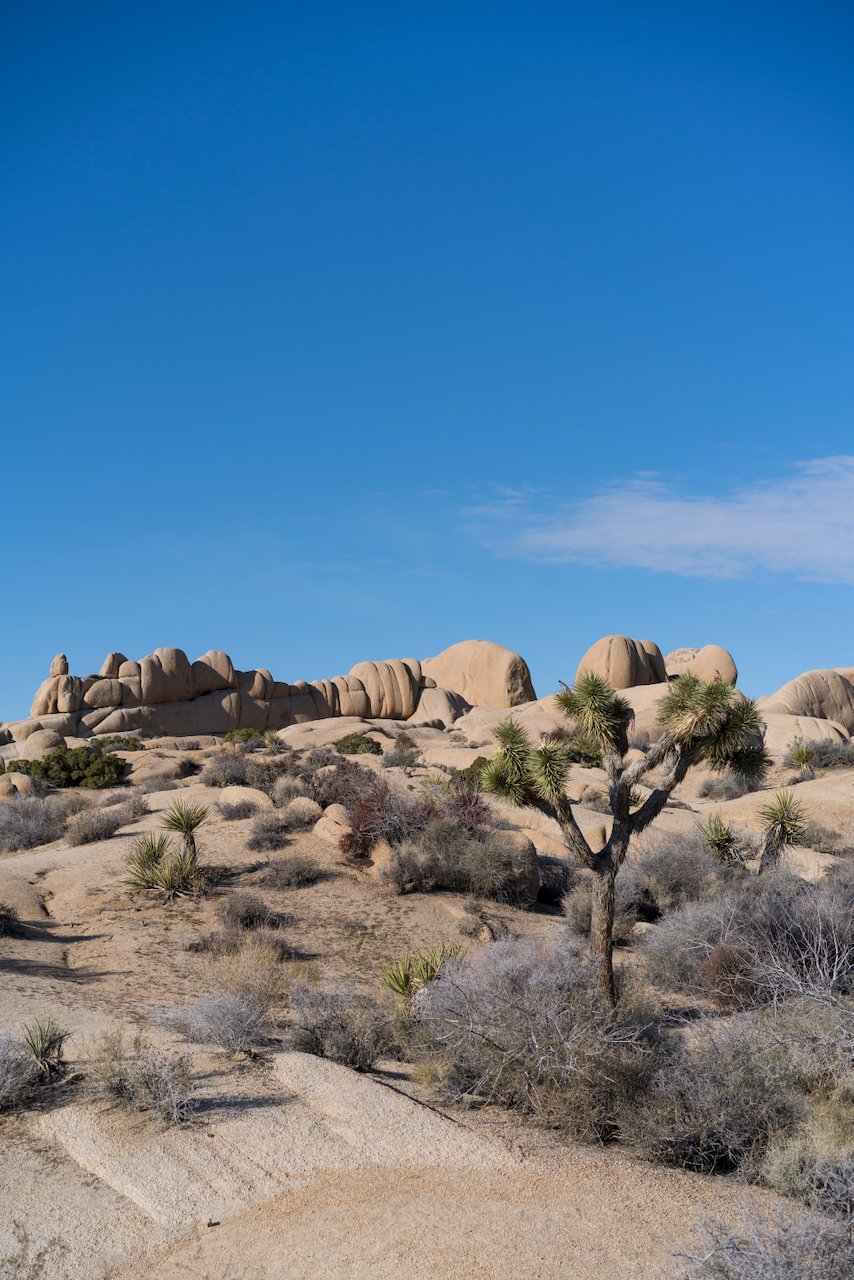
\includegraphics[width=\textwidth]{../Resource/image.png}
        \caption{Original}
        \label{fig:image-linear-bsc-original}
    \end{subfigure}
    \hfill
    \begin{subfigure}[b]{0.32\textwidth}
        \centering
        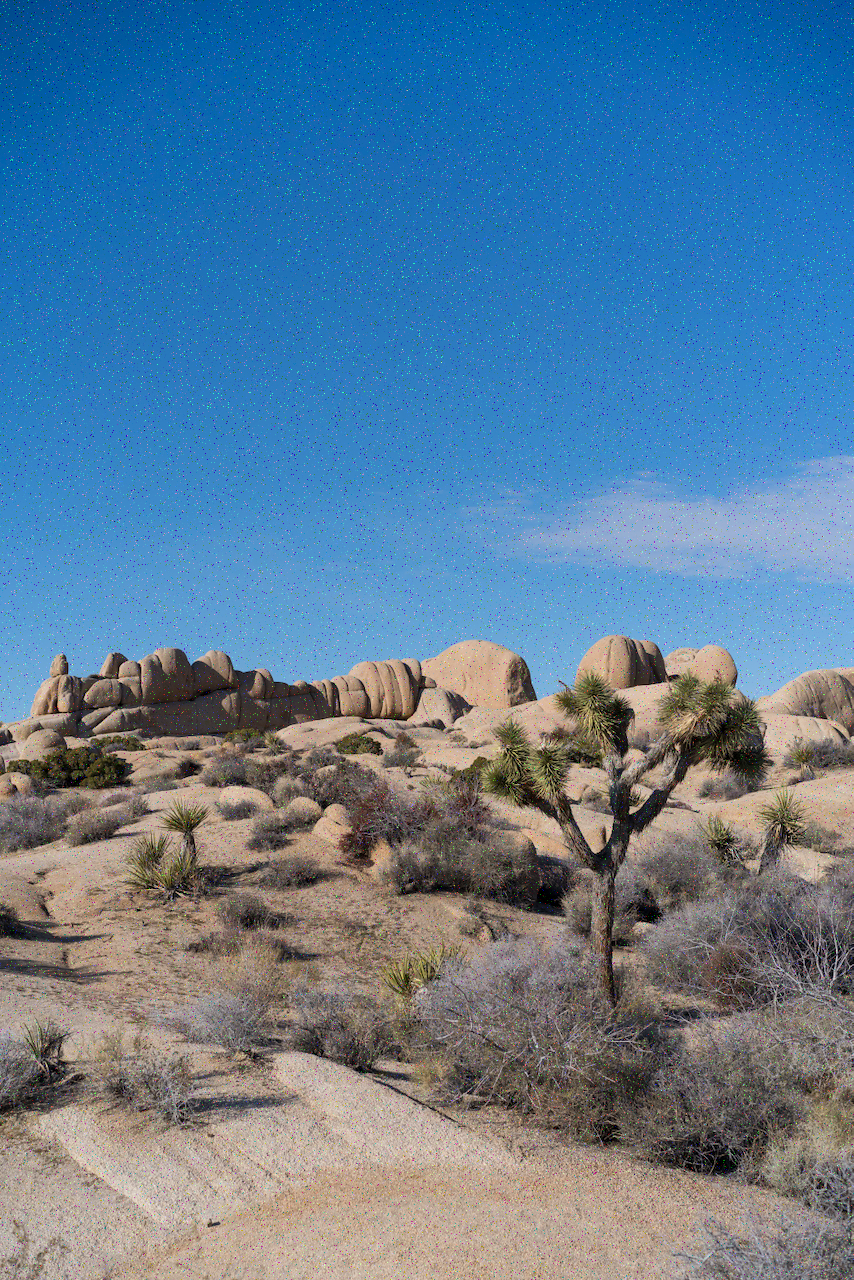
\includegraphics[width=\textwidth]{../Result/linear-bsc-output.png}
        \caption{Without correction}
        \label{fig:image-linear-bsc-no-correction}
    \end{subfigure}
    \hfill
    \begin{subfigure}[b]{0.32\textwidth}
        \centering
        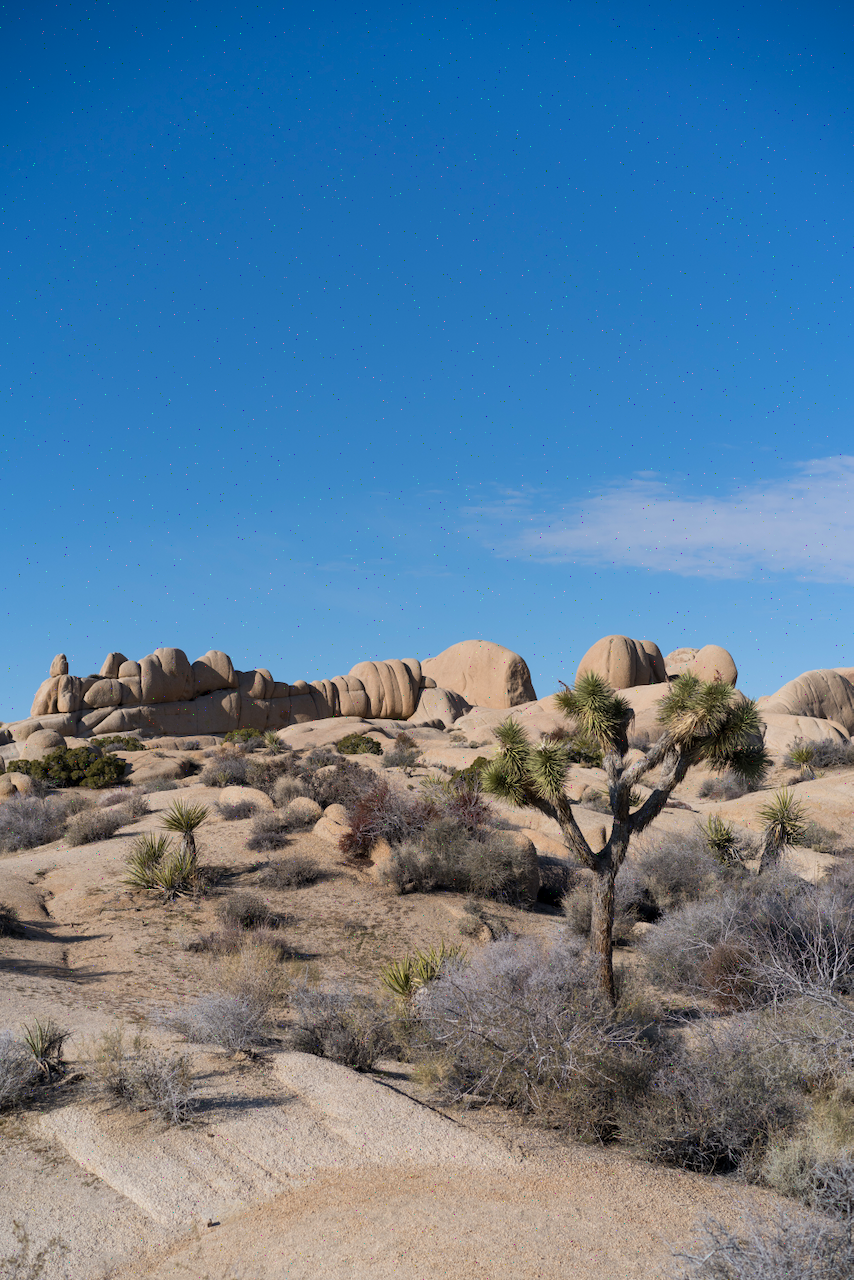
\includegraphics[width=\textwidth]{../Result/linear-bsc-output-syndrome-corrected.png}
        \caption{Corrected}
        \label{fig:image-linear-bsc-syndrome-corrected}
    \end{subfigure}
       \caption{Image encoded with Linear Hamming passed through BSC (entire)}
       \label{fig:image-linear-bsc}
\end{figure}


\begin{figure}
    \centering
    \begin{subfigure}[b]{0.32\textwidth}
        \centering
        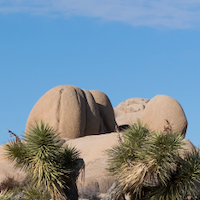
\includegraphics[width=\textwidth]{../Resource/cropped-image.png}
        \caption{Original}
        \label{fig:cropped-image-linear-bsc-original}
    \end{subfigure}
    \hfill
    \begin{subfigure}[b]{0.32\textwidth}
        \centering
        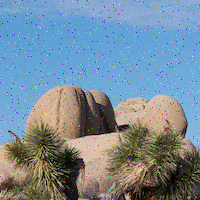
\includegraphics[width=\textwidth]{../Result/cropped-linear-bsc-output.png}
        \caption{Without correction}
        \label{fig:cropped-image-linear-bsc-no-correction}
    \end{subfigure}
    \hfill
    \begin{subfigure}[b]{0.32\textwidth}
        \centering
        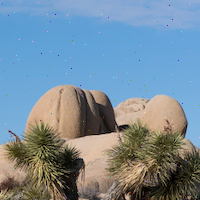
\includegraphics[width=\textwidth]{../Result/cropped-linear-bsc-output-syndrome-corrected.png}
        \caption{Corrected}
        \label{fig:cropped-image-linear-bsc-syndrome-corrected}
    \end{subfigure}
       \caption{Image encoded with Linear Hamming passed through BSC (details)}
       \label{fig:cropped-image-linear-bsc}
\end{figure}


\subsubsection{Audio}


\begin{figure}
    \centering
    \begin{subfigure}[b]{\textwidth}
        \centering
        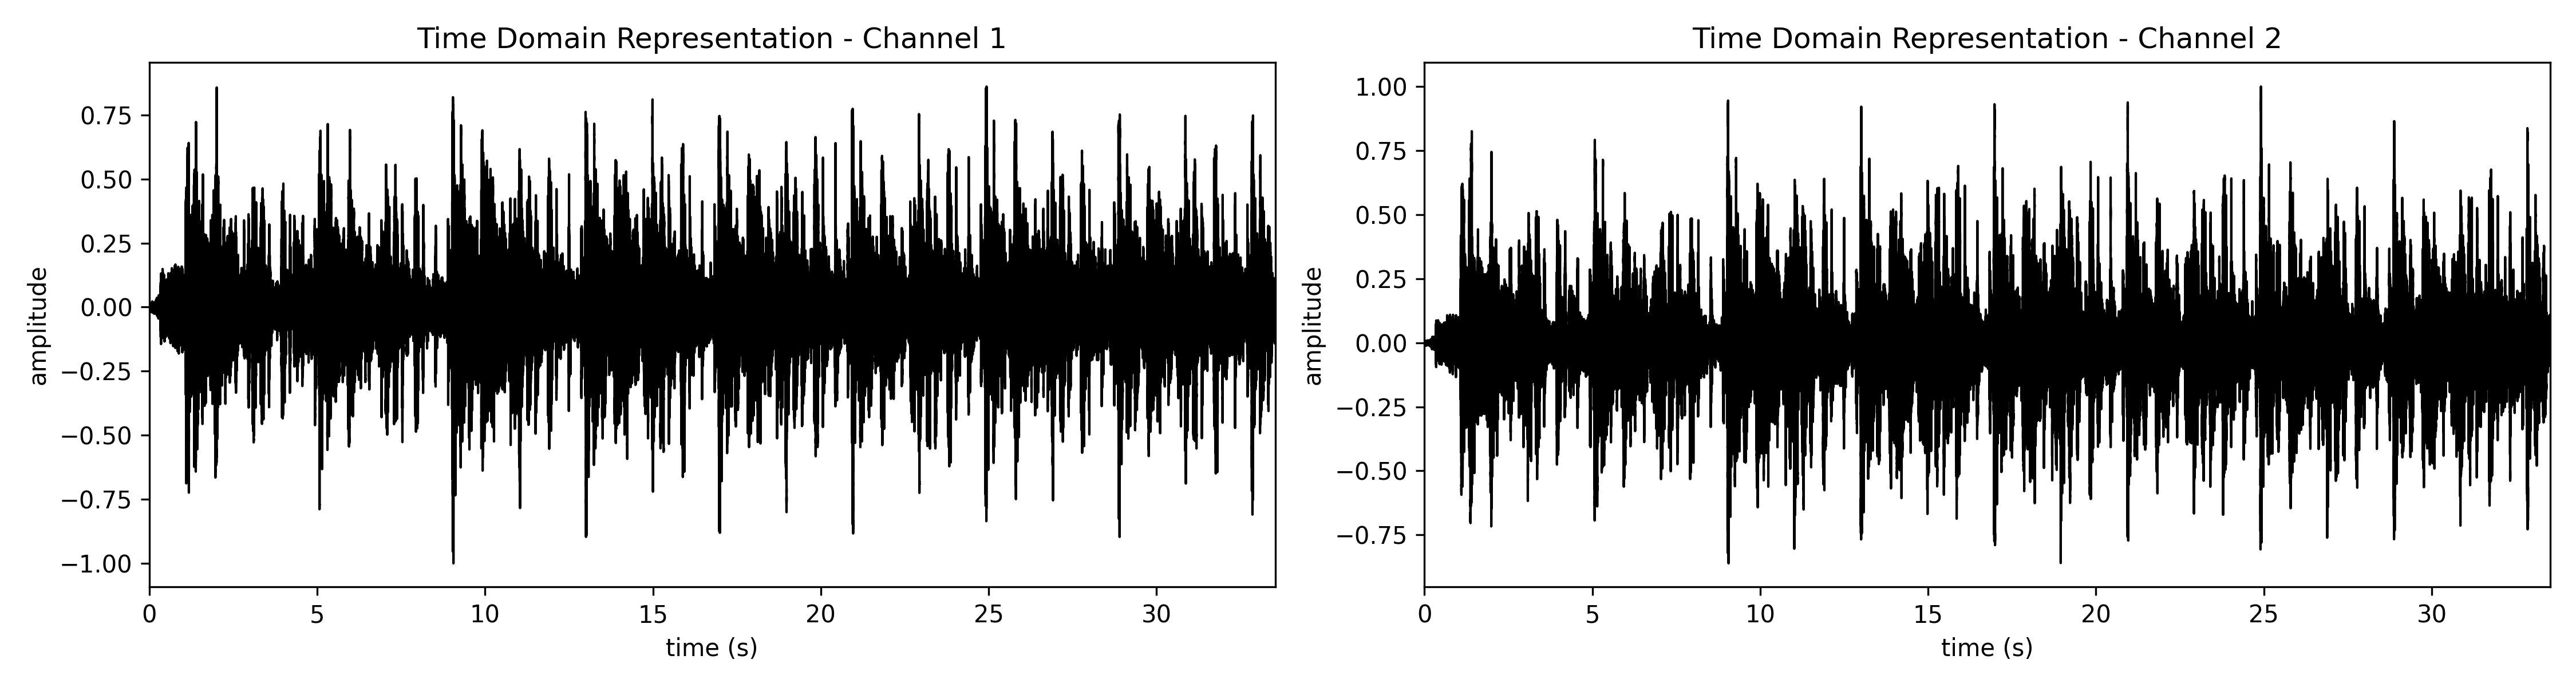
\includegraphics[width=\textwidth]{../Result/wav-time-domain-TX.png}
        \caption{Original}
        \label{fig:t-audio-linear-bsc-original}
    \end{subfigure}
    % \hfill
    \begin{subfigure}[b]{\textwidth}
        \centering
        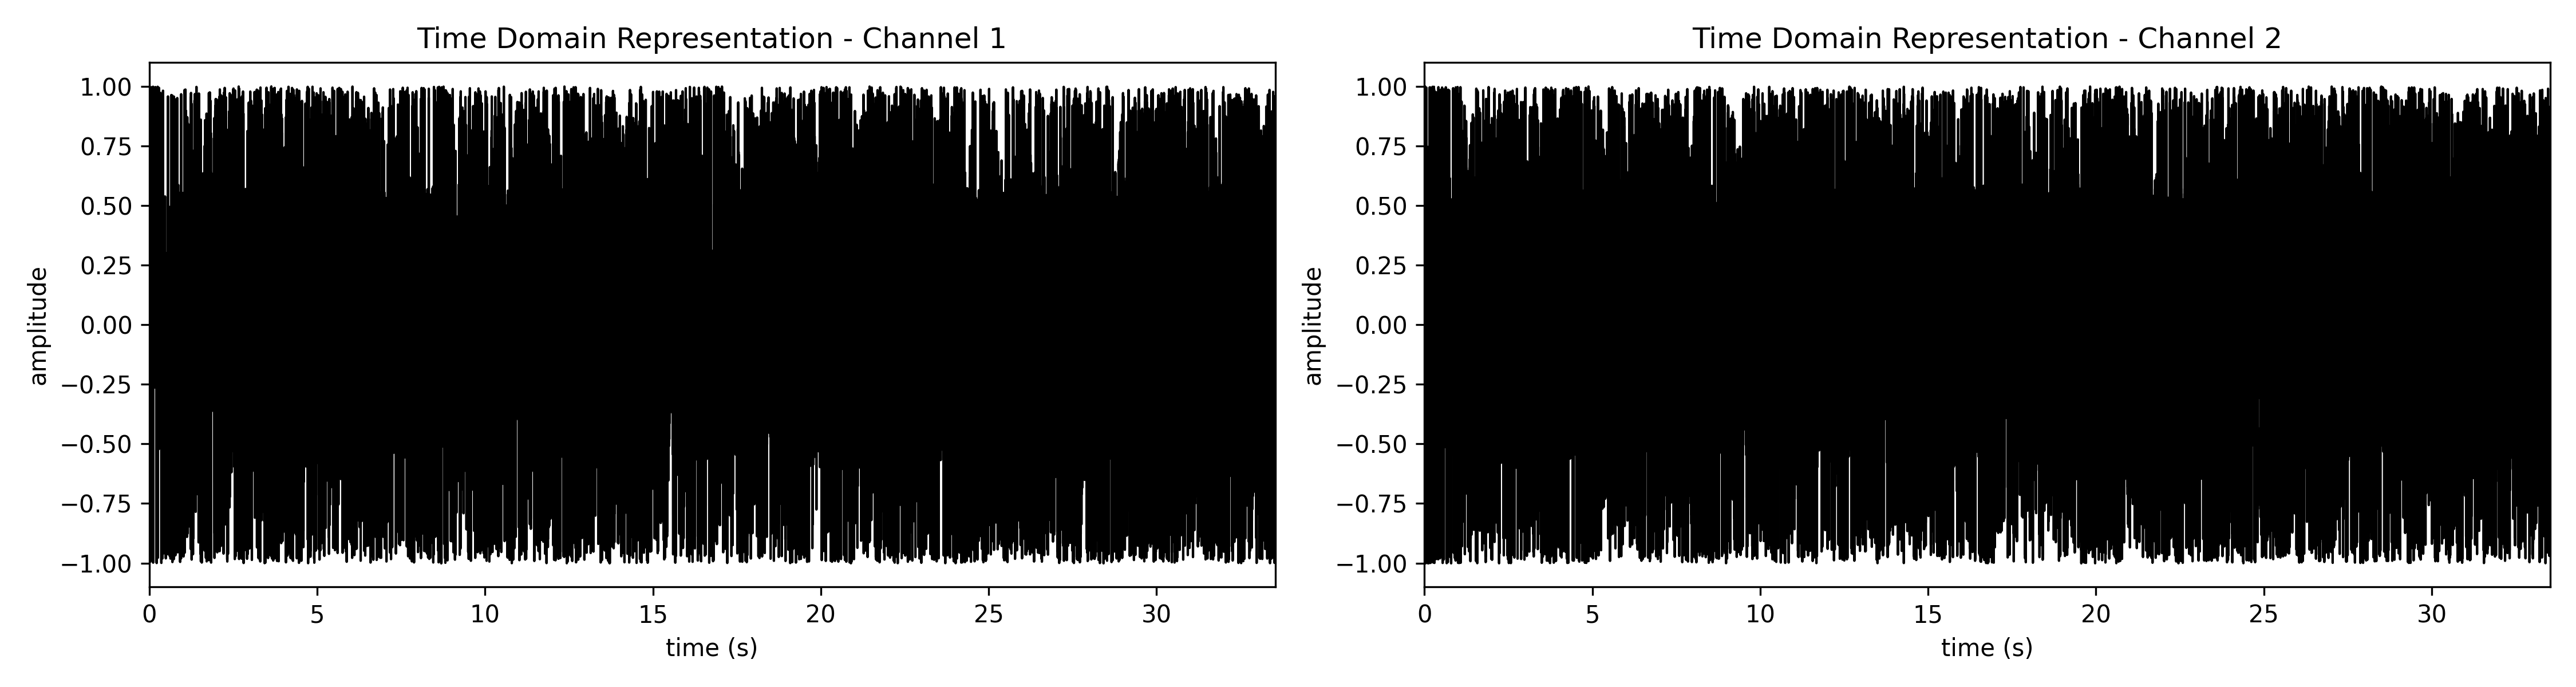
\includegraphics[width=\textwidth]{../Result/linear-bsc-wav-time-domain-RX.png}
        \caption{Without correction}
        \label{fig:t-audio-linear-bsc-no-correction}
    \end{subfigure}
    % \hfill
    \begin{subfigure}[b]{\textwidth}
        \centering
        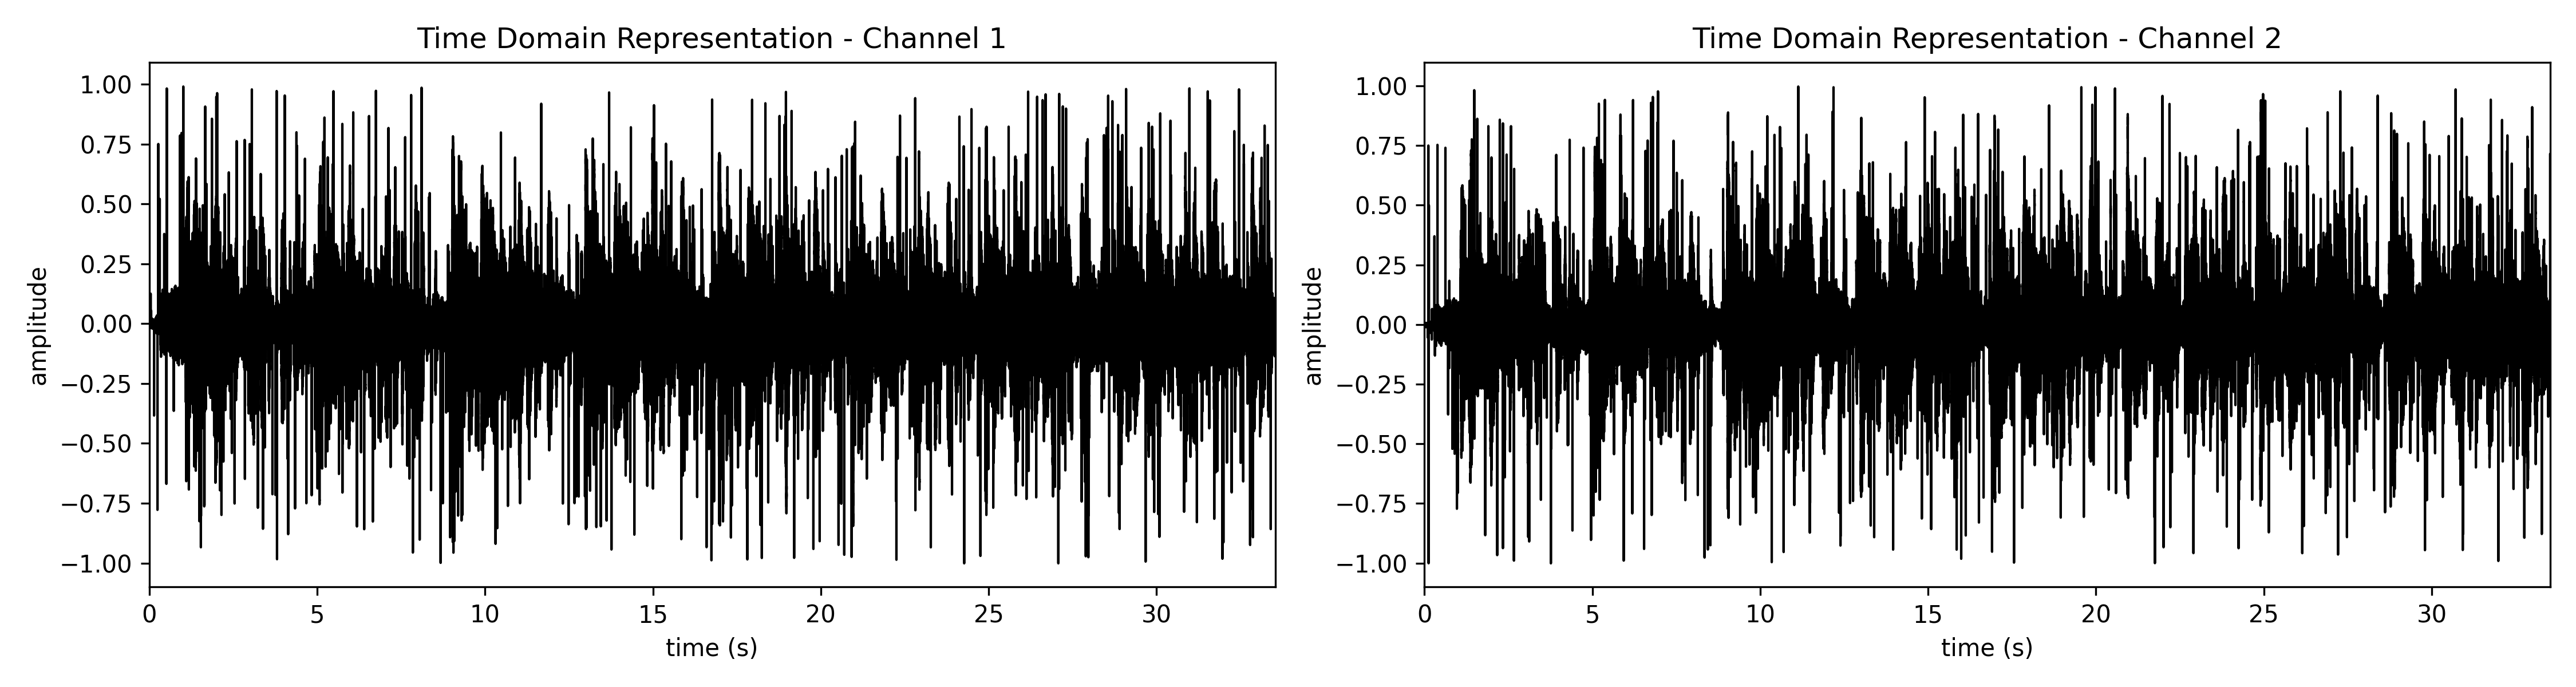
\includegraphics[width=\textwidth]{../Result/linear-bsc-wav-time-domain-RX-syndrome-corrected.png}
        \caption{Corrected}
        \label{fig:t-audio-linear-bsc-syndrome-syndrome-corrected}
    \end{subfigure}
       \caption{Audio encoded with Linear Hamming passed through BSC}
       \label{fig:t-audio-linear-bsc}
\end{figure}


\begin{figure}
    \centering
    \begin{subfigure}[b]{\textwidth}
        \centering
        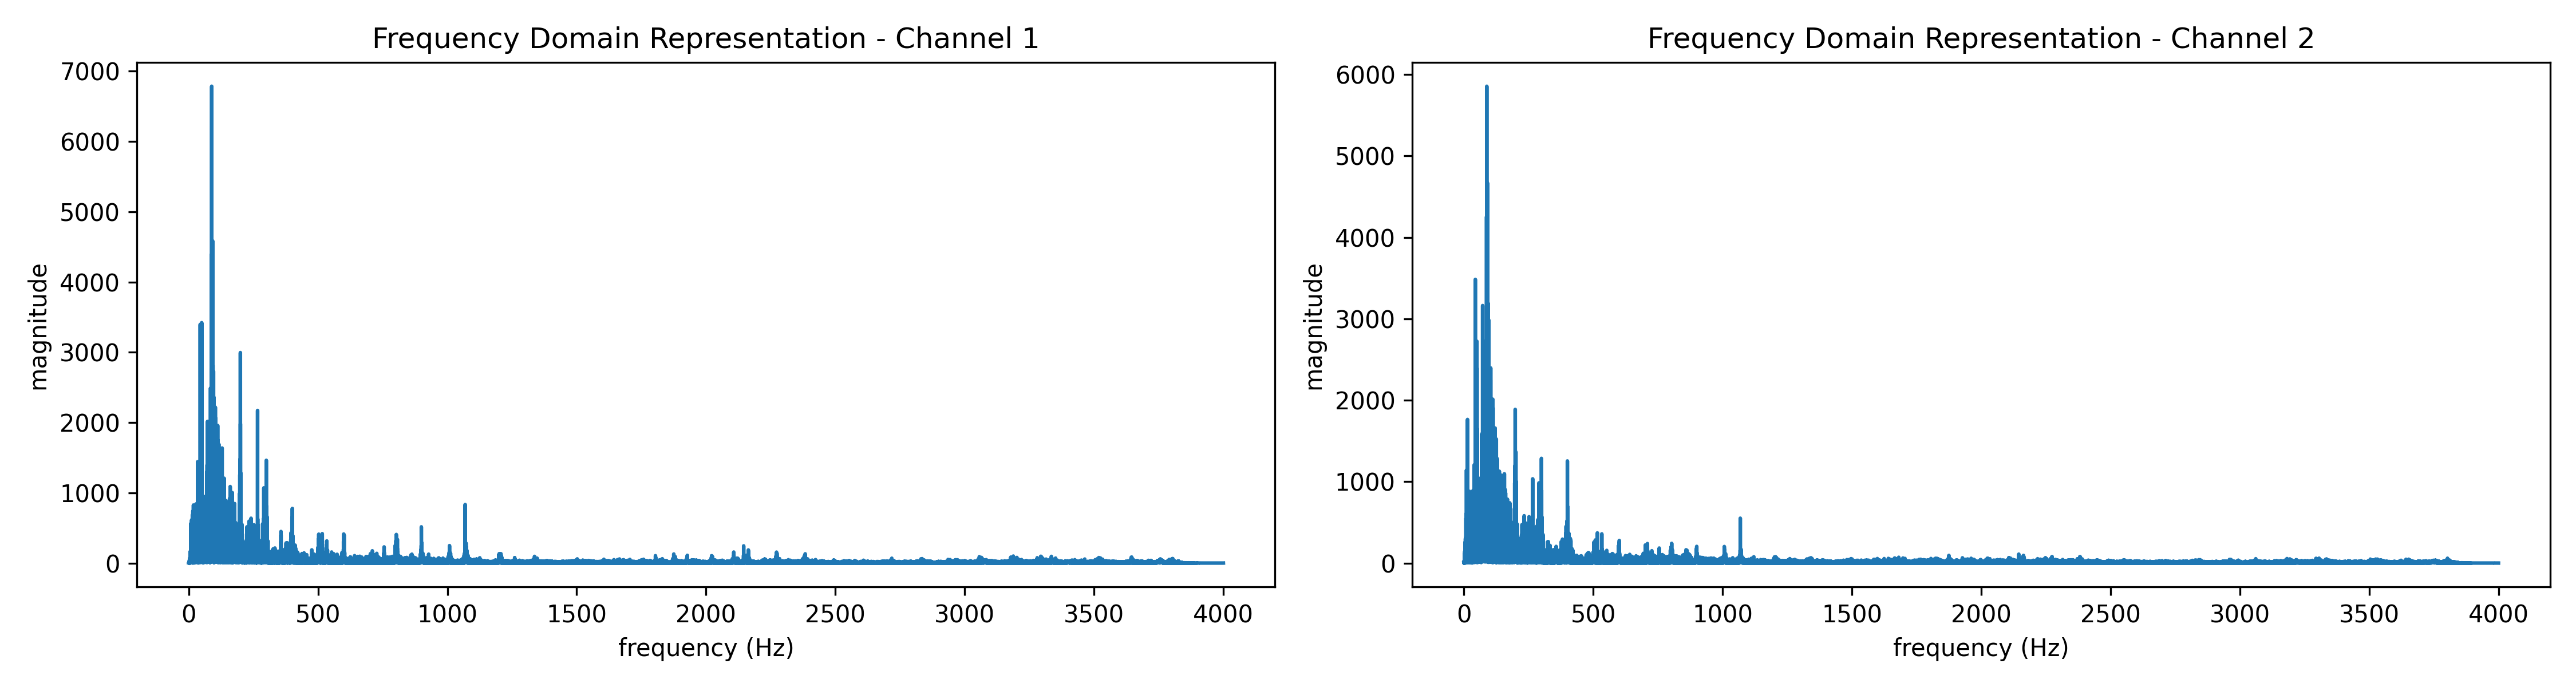
\includegraphics[width=\textwidth]{../Result/wav-frequency-domain-TX.png}
        \caption{Original}
        \label{fig:f-audio-linear-bsc-original}
    \end{subfigure}
    % \hfill
    \begin{subfigure}[b]{\textwidth}
        \centering
        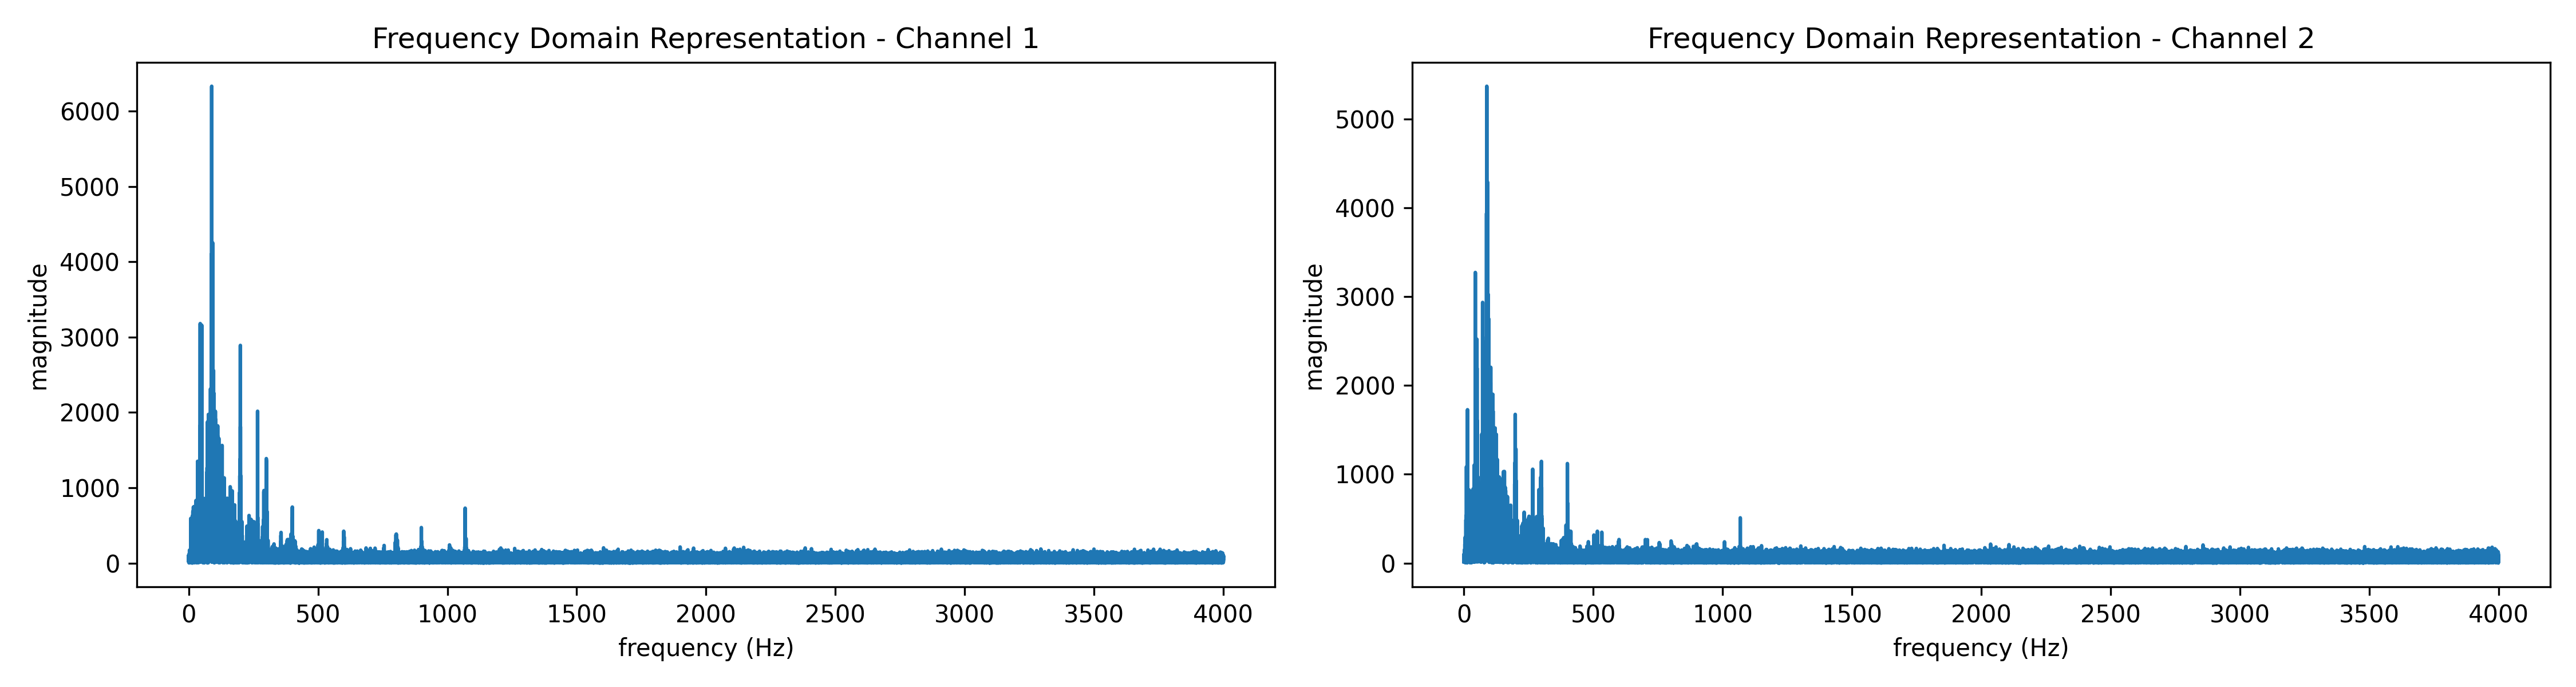
\includegraphics[width=\textwidth]{../Result/linear-bsc-wav-frequency-domain-RX.png}
        \caption{Without correction}
        \label{fig:f-audio-linear-bsc-no-correction}
    \end{subfigure}
    % \hfill
    \begin{subfigure}[b]{\textwidth}
        \centering
        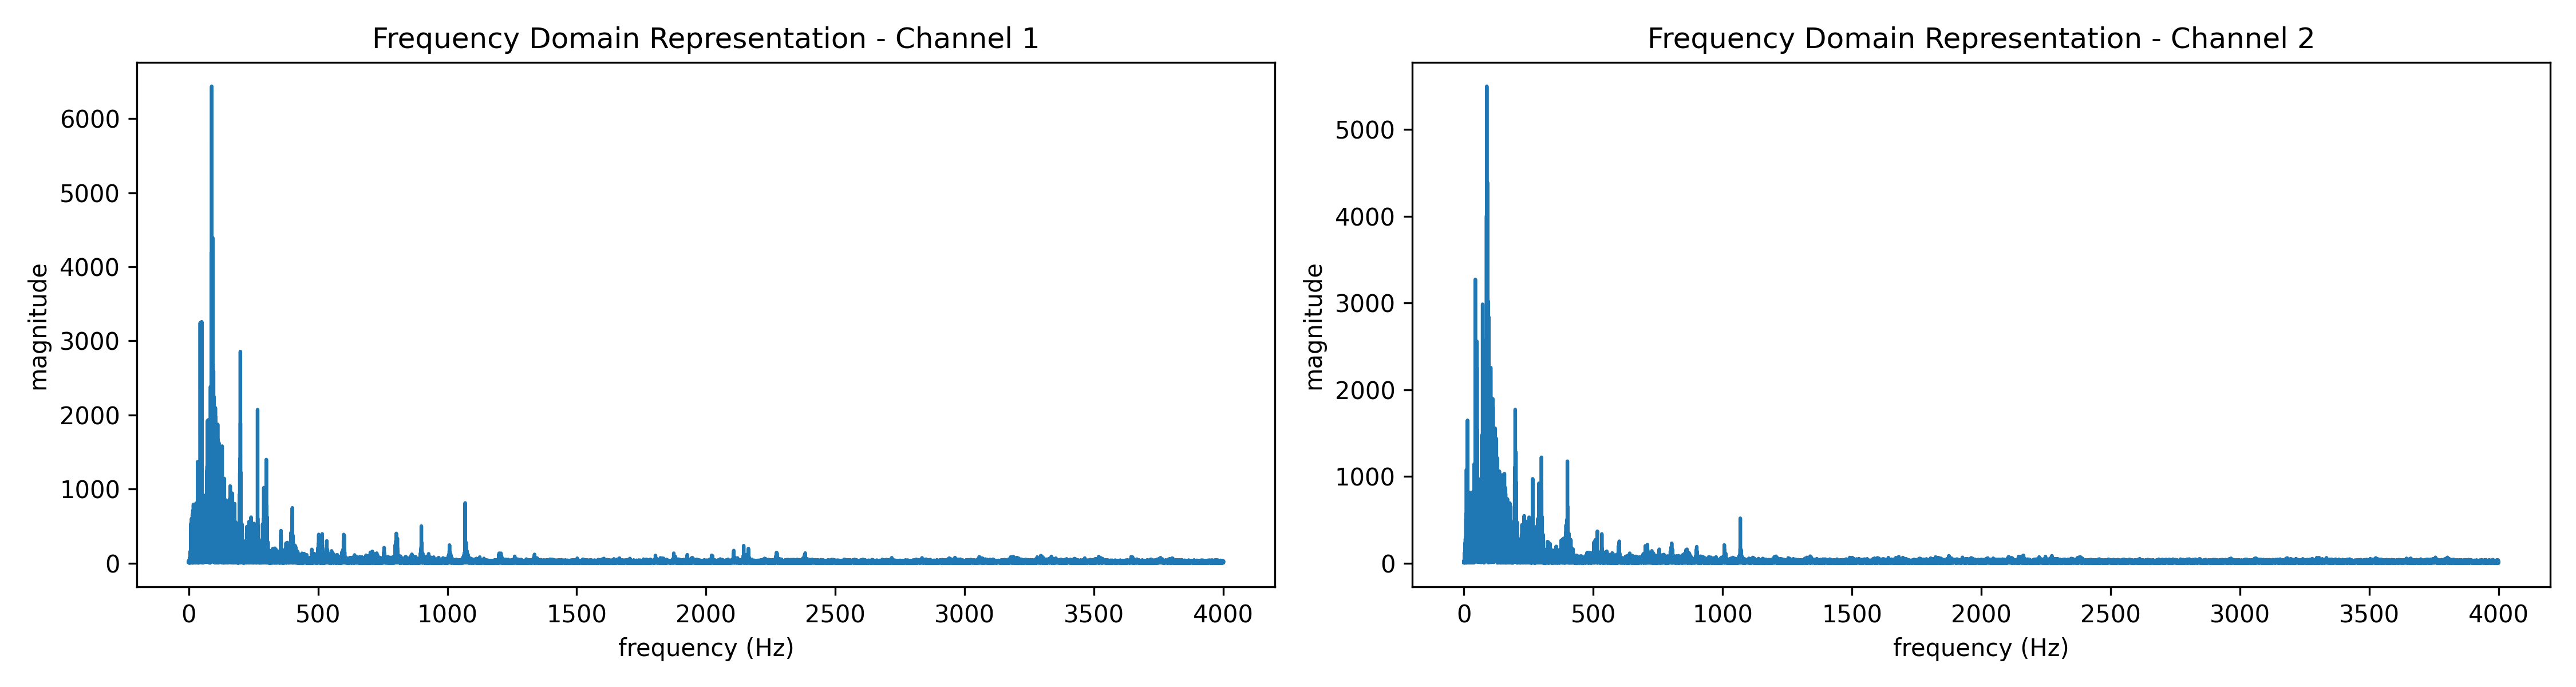
\includegraphics[width=\textwidth]{../Result/linear-bsc-wav-frequency-domain-RX-syndrome-corrected.png}
        \caption{Corrected}
        \label{fig:f-audio-linear-bsc-syndrome-corrected}
    \end{subfigure}
       \caption{Audio encoded with Linear Hamming passed through BSC}
       \label{fig:f-audio-linear-bsc}
\end{figure}


\section{$(n,k)$ Systematic Cyclic (Hamming) Code}
\subsection{Syndrome Decoder}
\subsubsection{Text string}


\begin{center}
    \renewcommand{\arraystretch}{1.5}
    \begin{tabulary}{\textwidth}{ |L|L|L| } 
    \hline
    \textbf{Original} & \textbf{Without correction} & \textbf{Corrected} \\
    \hline
    Hello World! EEC269A Error Correcting Code Demo & H\textcolor{red}{u,}lo World! EEC269A Error Correcti\textcolor{red}{f}g Code Demo & Hello World! EEC269A Error Correcting Code Demo \\
    \hline
    \end{tabulary}
\end{center}



\subsubsection{Image}


\begin{figure}
    \centering
    \begin{subfigure}[b]{0.32\textwidth}
        \centering
        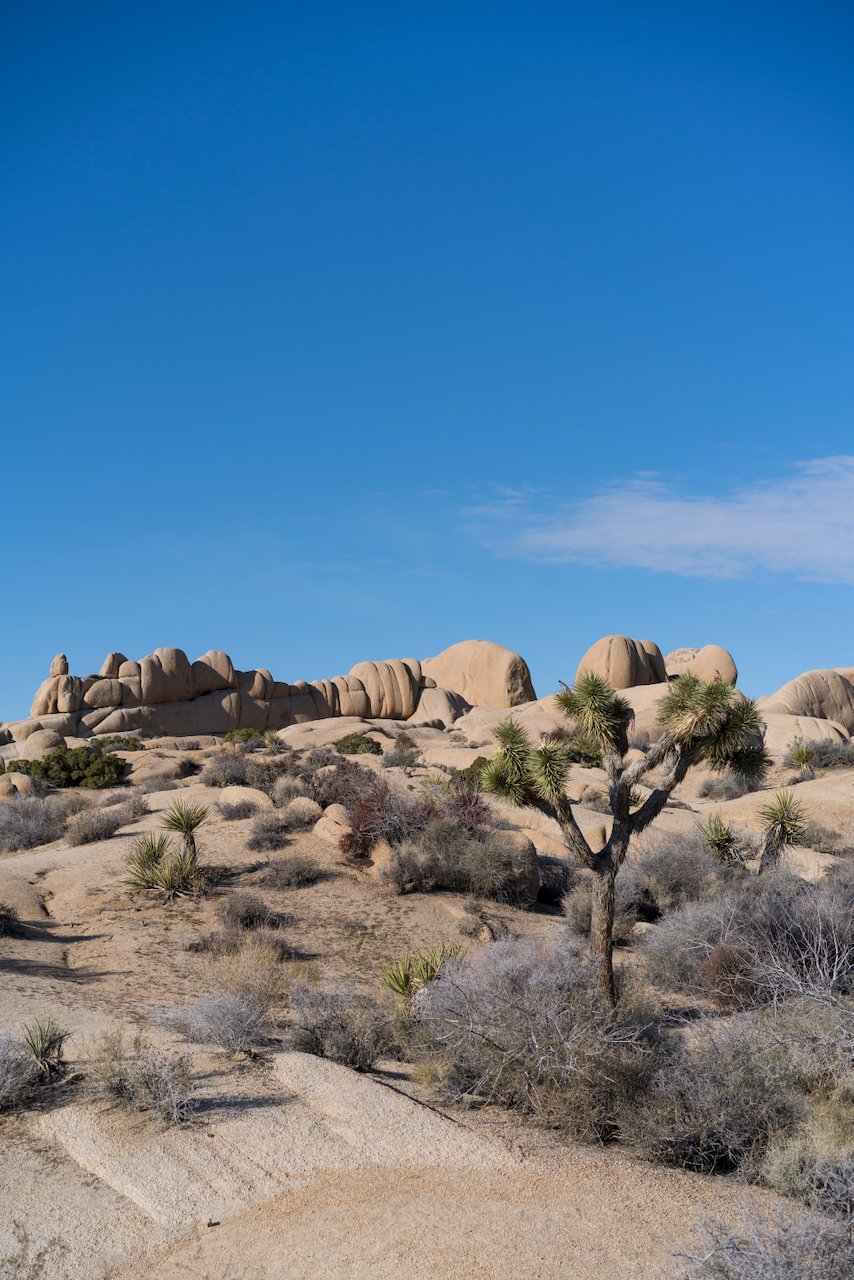
\includegraphics[width=\textwidth]{../Resource/image.png}
        \caption{Original}
        \label{fig:image-cyclic-bsc-original}
    \end{subfigure}
    \hfill
    \begin{subfigure}[b]{0.32\textwidth}
        \centering
        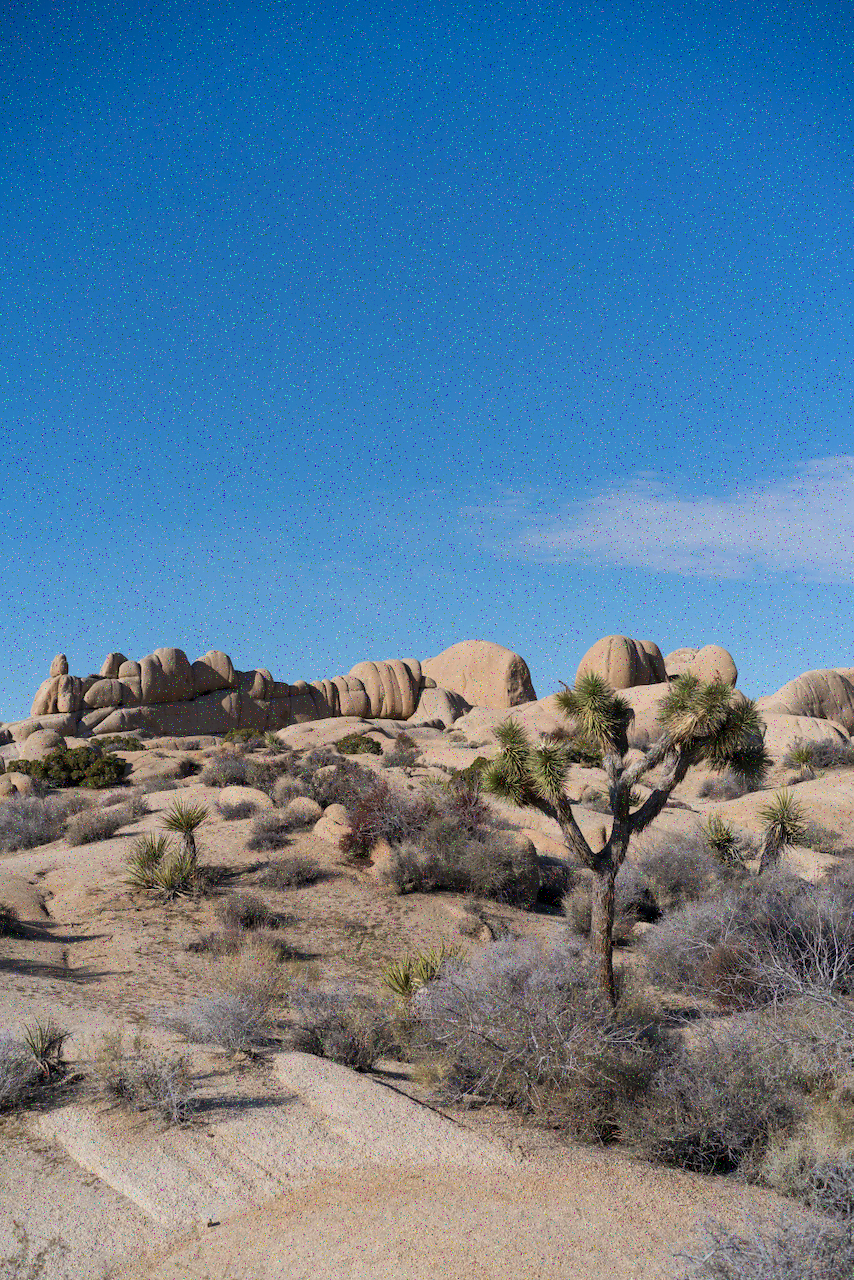
\includegraphics[width=\textwidth]{../Result/cyclic-bsc-output.png}
        \caption{Without correction}
        \label{fig:image-cyclic-bsc-no-correction}
    \end{subfigure}
    \hfill
    \begin{subfigure}[b]{0.32\textwidth}
        \centering
        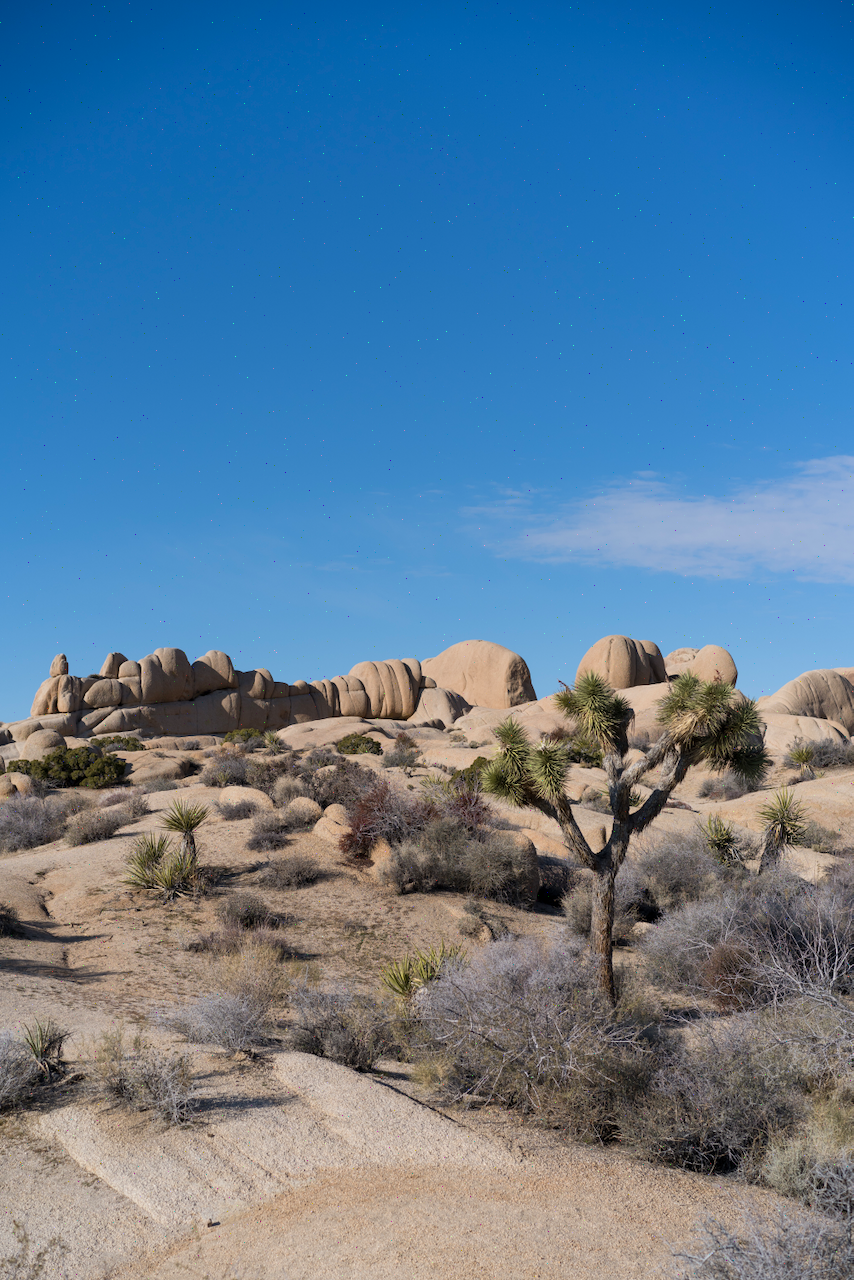
\includegraphics[width=\textwidth]{../Result/cyclic-bsc-output-syndrome-corrected.png}
        \caption{Corrected}
        \label{fig:image-cyclic-bsc-syndrome-corrected}
    \end{subfigure}
       \caption{Image encoded with Cyclic Hamming passed through BSC (entire)}
       \label{fig:image-cyclic-bsc}
\end{figure}




\begin{figure}
    \centering
    \begin{subfigure}[b]{0.32\textwidth}
        \centering
        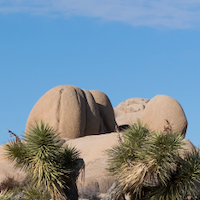
\includegraphics[width=\textwidth]{../Resource/cropped-image.png}
        \caption{Original}
        \label{fig:cropped-image-cyclic-bsc-original}
    \end{subfigure}
    \hfill
    \begin{subfigure}[b]{0.32\textwidth}
        \centering
        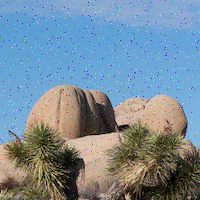
\includegraphics[width=\textwidth]{../Result/cropped-cyclic-bsc-output.png}
        \caption{Without correction}
        \label{fig:cropped-image-cyclic-bsc-no-correction}
    \end{subfigure}
    \hfill
    \begin{subfigure}[b]{0.32\textwidth}
        \centering
        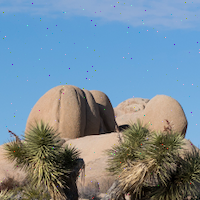
\includegraphics[width=\textwidth]{../Result/cropped-cyclic-bsc-output-syndrome-corrected.png}
        \caption{Corrected}
        \label{fig:cropped-image-cyclic-bsc-syndrome-corrected}
    \end{subfigure}
       \caption{Image encoded with Cyclic Hamming passed through BSC (details)}
       \label{fig:cropped-image-cyclic-bsc}
\end{figure}






\subsubsection{Audio}



\begin{figure}
    \centering
    \begin{subfigure}[b]{\textwidth}
        \centering
        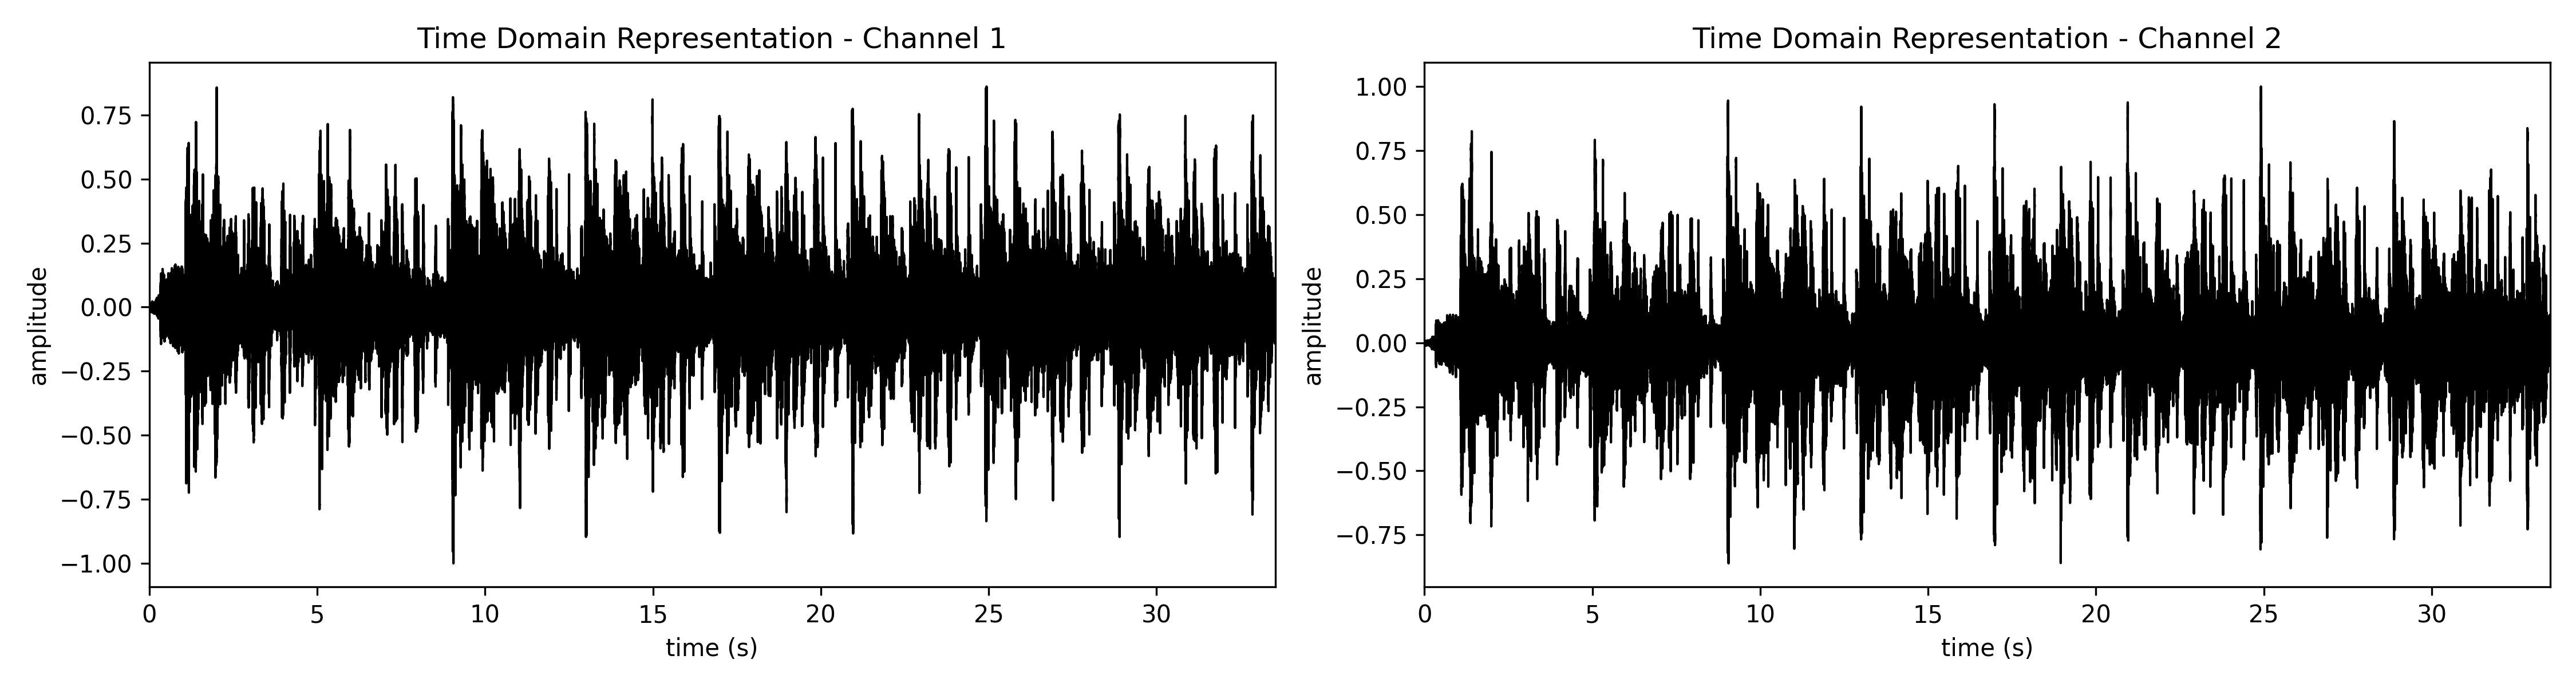
\includegraphics[width=\textwidth]{../Result/wav-time-domain-TX.png}
        \caption{Original}
        \label{fig:t-audio-cyclic-bsc-original}
    \end{subfigure}
    % \hfill
    \begin{subfigure}[b]{\textwidth}
        \centering
        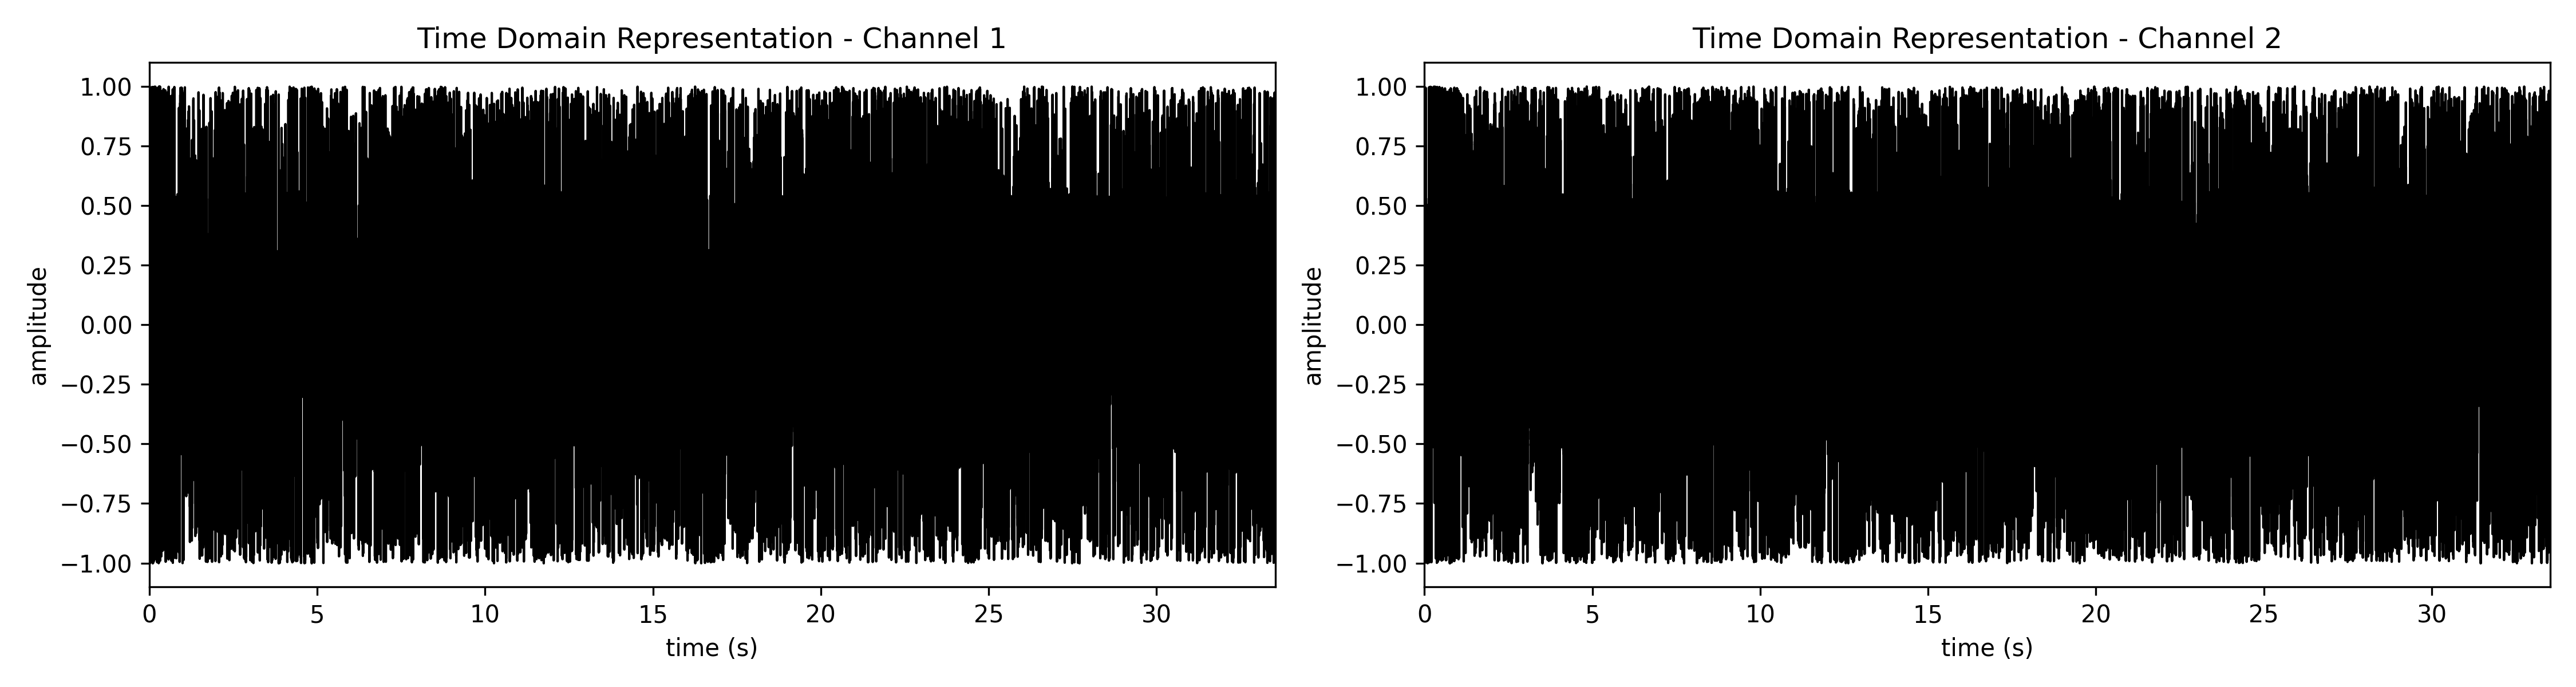
\includegraphics[width=\textwidth]{../Result/cyclic-bsc-wav-time-domain-RX.png}
        \caption{Without correction}
        \label{fig:t-audio-cyclic-bsc-no-correction}
    \end{subfigure}
    % \hfill
    \begin{subfigure}[b]{\textwidth}
        \centering
        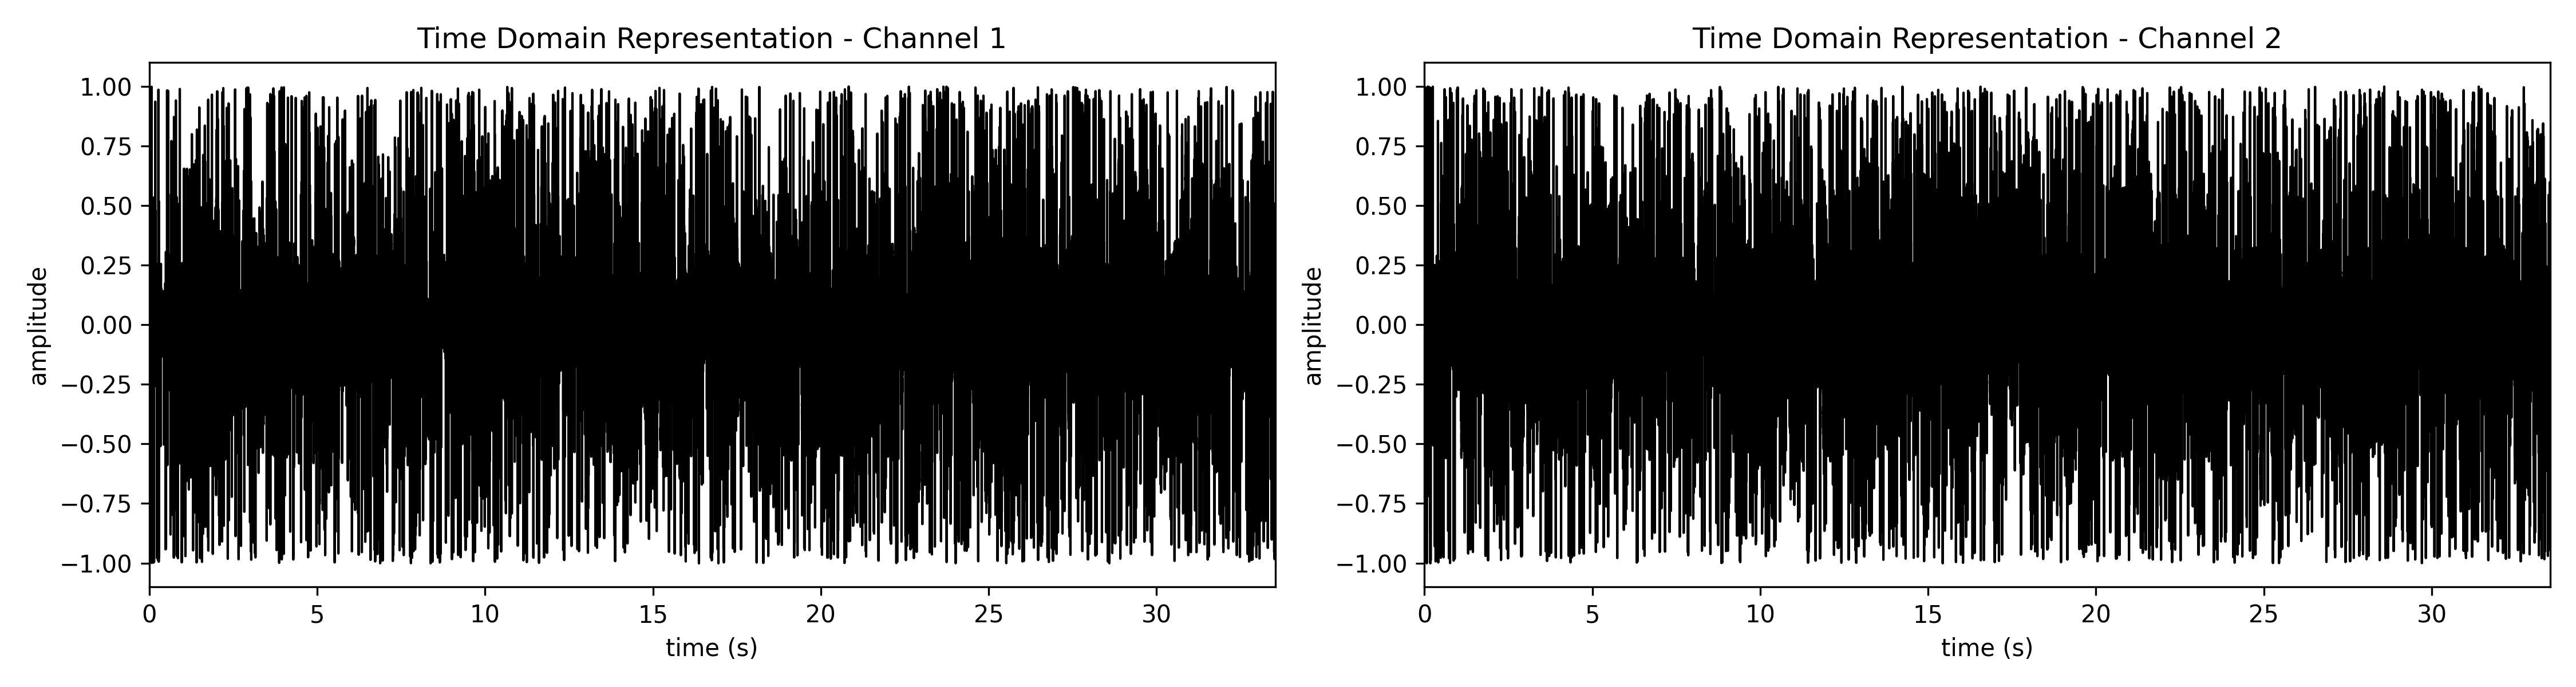
\includegraphics[width=\textwidth]{../Result/cyclic-bsc-wav-time-domain-RX-syndrome-corrected.png}
        \caption{Corrected}
        \label{fig:t-audio-cyclic-bsc-syndrome-syndrome-corrected}
    \end{subfigure}
       \caption{Audio encoded with Cyclic Hamming passed through BSC}
       \label{fig:t-audio-cyclic-bsc}
\end{figure}



\begin{figure}
    \centering
    \begin{subfigure}[b]{\textwidth}
        \centering
        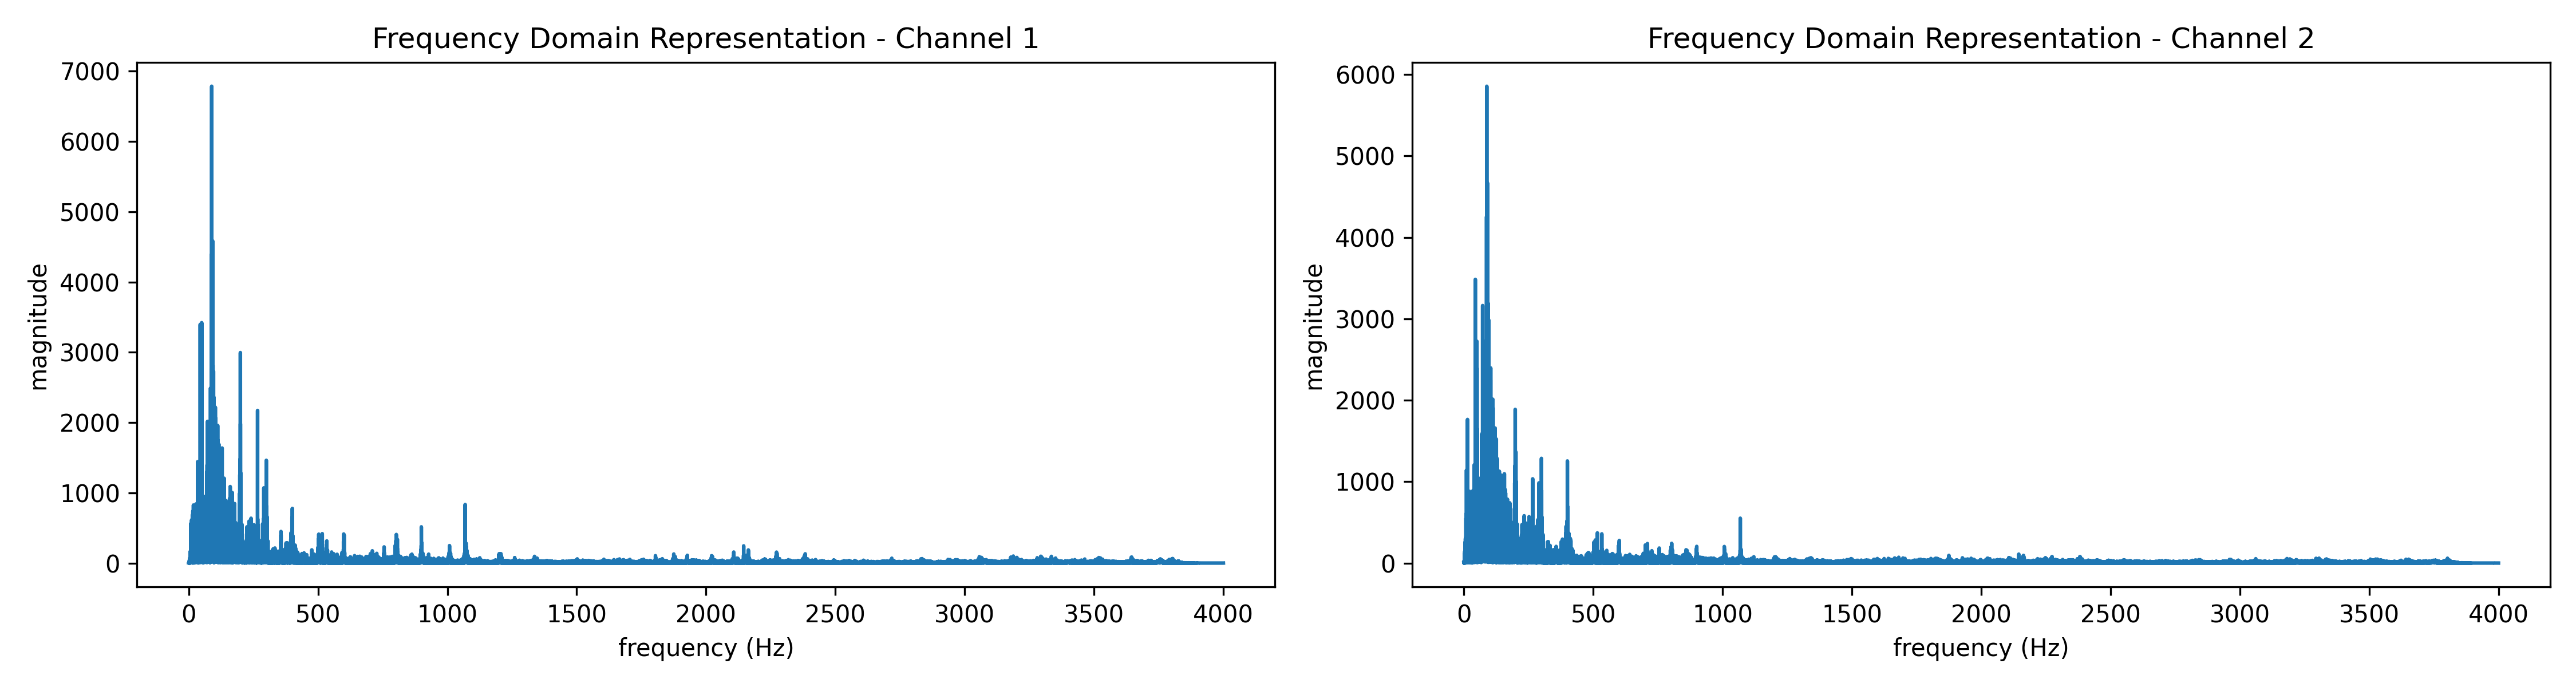
\includegraphics[width=\textwidth]{../Result/wav-frequency-domain-TX.png}
        \caption{Original}
        \label{fig:f-audio-cyclic-bsc-original}
    \end{subfigure}
    % \hfill
    \begin{subfigure}[b]{\textwidth}
        \centering
        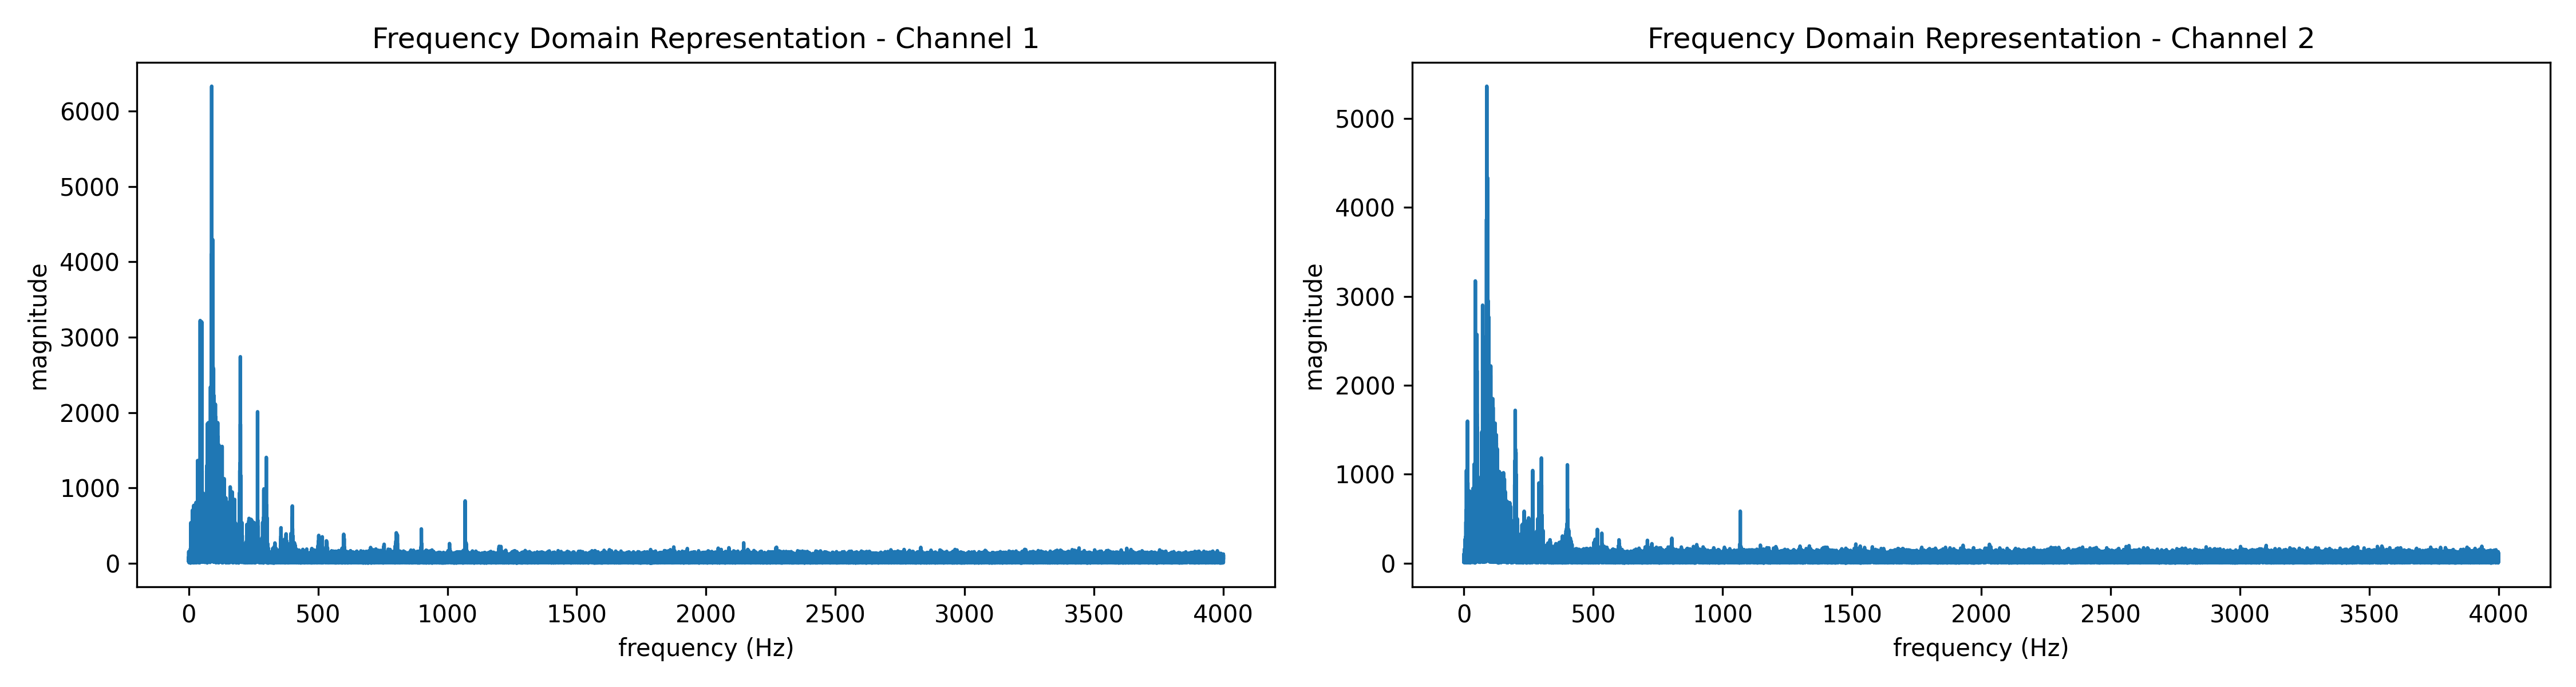
\includegraphics[width=\textwidth]{../Result/cyclic-bsc-wav-frequency-domain-RX.png}
        \caption{Without correction}
        \label{fig:f-audio-cyclic-bsc-no-correction}
    \end{subfigure}
    % \hfill
    \begin{subfigure}[b]{\textwidth}
        \centering
        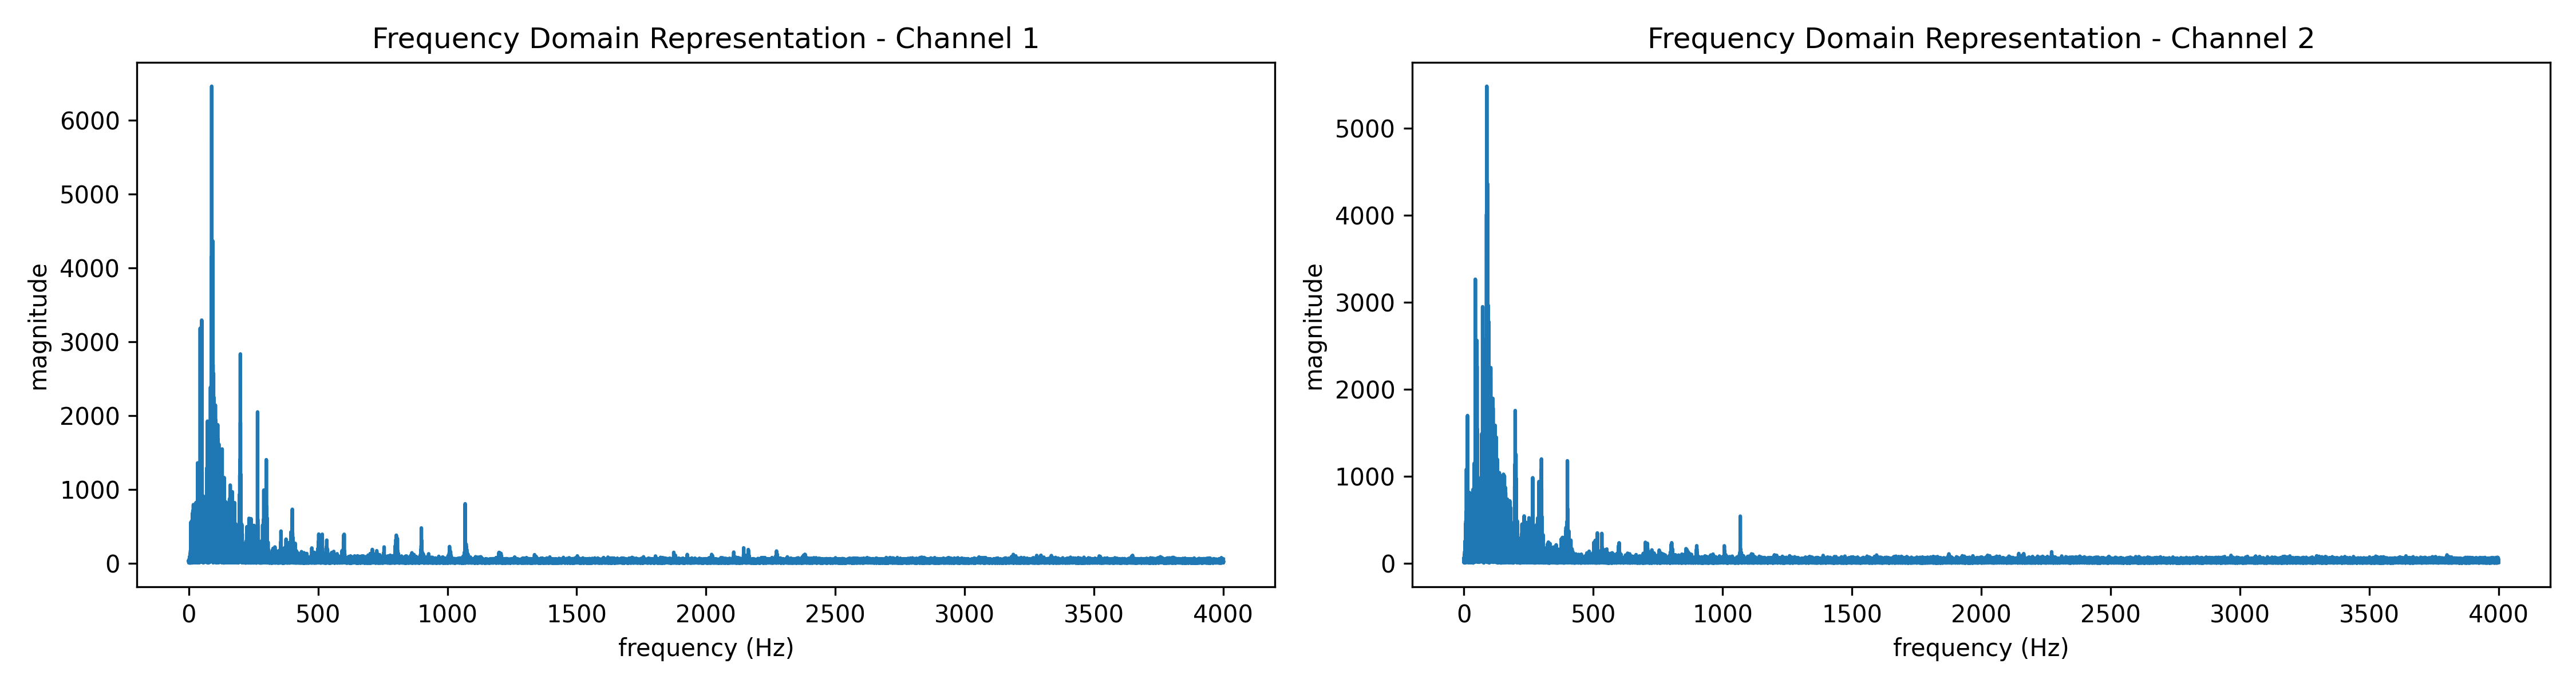
\includegraphics[width=\textwidth]{../Result/cyclic-bsc-wav-frequency-domain-RX-syndrome-corrected.png}
        \caption{Corrected}
        \label{fig:f-audio-cyclic-bsc-syndrome-corrected}
    \end{subfigure}
       \caption{Audio encoded with Cyclic Hamming passed through BSC}
       \label{fig:f-audio-cyclic-bsc}
\end{figure}






\subsection{LFSR Decoder}


\newpage
\section{Appendix: Python source code}
\subsection{Source}
\label{appendix:source}
\lstinputlisting[language=Python]{../Code/Source/source.py}

\subsection{Channel}
\label{appendix:channel}
\lstinputlisting[language=Python]{../Code/Channel/channel.py}

\subsection{Destination}
\label{appendix:destination}
\lstinputlisting[language=Python]{../Code/Destination/destination.py}

\subsection{Utilities}
\label{appendix:utils}
\lstinputlisting[language=Python]{../Code/Utils/plot_wav.py}
\lstinputlisting[language=Python]{../Code/Utils/polyTools.py}

\subsection{Linear code}
\label{appendix:linear-code}
\lstinputlisting[language=Python]{../Code/linear-code.py}

\subsection{Cyclic code}
\label{appendix:cyclic-code}
\lstinputlisting[language=Python]{../Code/cyclic-code.py}


\end{document}